% Drawing 144/07-6 -- folder 144, batch 07, archive page 133 (PDF page 134).
% Transcription: un cube d'inclusions : face avant $\mu\times\mu_\tau = D_2 \overset{2}{\hookrightarrow} \mu\times\Pi'_0 = \mathfrak{S}^! = \Pi^!_0$ (lecture incertaine) $\overset{6}{\hookrightarrow}\mathfrak{S}$ ; $\mu_\tau\overset{2}{\hookrightarrow}\mathfrak{S}^!_0 = \Pi'$ ; face arrière $\underline\mu \overset{2}{\hookrightarrow} \mu\times\Pi_0 = \mathfrak{S}^{!+} = \Pi \overset{6}{\hookrightarrow} \underline{\mathfrak{S}}^+$, $\{1\}\overset{2}{\hookrightarrow}\mathfrak{S}^{!+}_0 = \Pi_0$ ; toutes les arêtes verticales et diagonales d'indice 2 ; $\mathfrak{S}$ et $\mathfrak{S}^+$ reliés par un trait d'indice 2. Une ligne courbe sépare ce cube de la partie (I).
% Kind: cube of inclusions (II), with the separating curve. Method 2 (schematic redraw from the facsimile). Status: partial.
% Notes: Re-read on a tight crop. Cube (II): front face D_2 -2-> S^! -6-> S and mu -2-> S^{!+} -6-> S^+; inner square mu_tau -2-> S^!_0 = Pi' and {1} -2-> S^{!+}_0 = Pi_0; the diagonals mu_tau -> D_2, S^!_0 -> S^!, {1} -> mu, S^{!+}_0 -> S^{!+}, the verticals mu -- D_2, {1} -- mu_tau, S^{!+}_0 -> S^!_0, S^{!+} -- S^!, S^+ -> S, each with the index he writes (2 or 6), \small, where he wrote it. The node names are now given in full as on the page: mu x mu_tau = D_2, S^! = Pi^!_0 with mu x Pi'_0 = written under it, S^!_0 = Pi', S^{!+} = Pi with mu x Pi_0 = under it, S^{!+}_0 = Pi_0, underlined mu and S^+. The circled II and the curve separating the cube from part (I) are drawn. Still differs from the facsimile: hooks are drawn as plain arrows; the vertical S^{!+} -- S^! has an arrowhead at each end on the page (drawn so), the verticals mu -- D_2 and {1} -- mu_tau show no clear head and are plain; the reading S^! = Pi^!_0 stays uncertain, as in the transcription. The formulas at the right and the arrows to L_rho from part (I) above are not part of this figure. Redrawn 2026-11-09 (issue 128): to check again. Overlay check 2026-11-13 (issue 147, Claude Opus 5.5): the redraw, rasterised from its TikZ paths, laid over the 300 dpi colour render of the 250 ppi scan: every node label stands on its ink and every arrow on its stroke (98 % of the drawn length within 0.6 unit of ink). Nothing changed. Still differs, as listed above: the hooks are drawn as plain arrows, the heads of the verticals mu -- D_2 and {1} -- mu_tau are not legible, and the reading S^! = Pi^!_0 stays uncertain. A large arrow diagram (a cube), kept partial as the skill asks for them. Not compiled (no TeX engine in the session).
% Coordinates: 1 unit = 1 mm = 1/100 of the crop width (bbox in page fractions: [0.1, 0.49, 0.86, 0.7]).
% Redrawn by Claude (claude-opus-5-5), issue #73, 2026-11-09; not checked by a human; not compiled (no TeX in the session).
% Checked by Claude (claude-opus-5-5) 2026-11-13 (issue #147): overlay on the 300 dpi colour render of the 250 ppi scan; nothing changed; not compiled (no TeX in the session). Not checked by a human. Status: partial.
% Rights: reproduces part of the work -- behind RENDER_TRANSCRIPTS, never published by itself.
\documentclass[tikz,border=3pt]{standalone}
\usepackage{amsmath,amssymb}
\usetikzlibrary{patterns,arrows.meta}
\tikzset{pencil/.style={black!45}, struck/.style={black!35}, mark/.style={circle,draw,inner sep=1.3pt}, pt/.style={circle,fill,inner sep=0.9pt}, opt/.style={circle,draw,fill=white,inner sep=1.1pt}}
\begin{document}
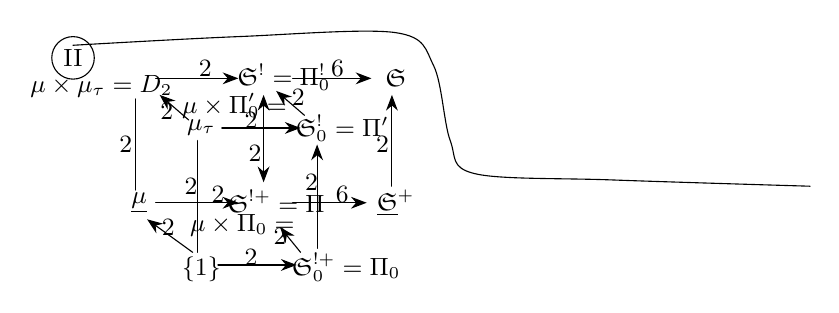
\begin{tikzpicture}[x=1mm,y=1mm,line cap=round,line join=round,font=\scriptsize]
\draw[-{Stealth[length=2mm]}] (15.8,-9.2) -- (26.3,-9.2);
\draw[-{Stealth[length=2mm]}] (33.2,-9.2) -- (43.2,-9.2);
\draw[-{Stealth[length=2mm]}] (24.2,-15.5) -- (34.2,-15.5);
\draw[-{Stealth[length=2mm]}] (20,-14.5) -- (16.3,-11.3);
\draw[-{Stealth[length=2mm]}] (34.7,-13.9) -- (31.1,-10.8);
\draw[{Stealth[length=2mm]}-{Stealth[length=2mm]}] (29.5,-22.4) -- (29.5,-11.3);
\draw[-{Stealth[length=2mm]}] (45.8,-22.9) -- (45.8,-11.3);
\draw (13.2,-23.4) -- (13.2,-11.8);
\draw[-{Stealth[length=2mm]}] (15.8,-25) -- (26.3,-25);
\draw[-{Stealth[length=2mm]}] (33.2,-25) -- (42.6,-25);
\draw[-{Stealth[length=2mm]}] (20.5,-31.3) -- (14.7,-27.1);
\draw[-{Stealth[length=2mm]}] (23.7,-32.9) -- (33.7,-32.9);
\draw[-{Stealth[length=2mm]}] (34.2,-31.3) -- (31.6,-28.1);
\draw[-{Stealth[length=2mm]}] (36.3,-30.8) -- (36.3,-17.6);
\draw (21.1,-31.3) -- (21.1,-17.1);
\draw plot[smooth, tension=0.55] coordinates {(5.3,-5) (26.3,-3.9) (46.3,-3.4) (51.1,-7.6) (53.2,-17.1) (56.3,-21.3) (73.7,-22.1) (98.9,-22.9)};
\draw (5.3,-6.6) circle[radius=2.7];
\node[inner sep=1pt] at (5.3,-6.6) {\small $\mathrm{II}$};
\node[inner sep=1pt] at (8.9,-10.2) {\small $\mu\times\mu_\tau=D_2$};
\node[inner sep=1pt] at (32.1,-9) {\small $\mathfrak{S}^!=\Pi^!_0$};
\node[inner sep=1pt] at (25.8,-12.7) {\small $\mu\times\Pi'_0=$};
\node[inner sep=1pt] at (46.3,-9.2) {\small $\mathfrak{S}$};
\node[inner sep=1pt] at (21.6,-15.5) {\small $\mu_\tau$};
\node[inner sep=1pt] at (39.5,-15.5) {\small $\mathfrak{S}^!_0=\Pi'$};
\node[inner sep=1pt] at (13.7,-25) {\small $\underline{\mu}$};
\node[inner sep=1pt] at (31.1,-24.8) {\small $\mathfrak{S}^{!+}=\Pi$};
\node[inner sep=1pt] at (26.8,-27.9) {\small $\mu\times\Pi_0=$};
\node[inner sep=1pt] at (46.3,-25) {\small $\underline{\mathfrak{S}}^+$};
\node[inner sep=1pt] at (21.6,-33.4) {\small $\{1\}$};
\node[inner sep=1pt] at (40,-33.2) {\small $\mathfrak{S}^{!+}_0=\Pi_0$};
\node[inner sep=1pt] at (22.1,-8) {\small $2$};
\node[inner sep=1pt] at (38.9,-8) {\small $6$};
\node[inner sep=1pt] at (27.9,-14.6) {\small $2$};
\node[inner sep=1pt] at (17.2,-13.4) {\small $2$};
\node[inner sep=1pt] at (33.9,-11.6) {\small $2$};
\node[inner sep=1pt] at (28.4,-18.7) {\small $2$};
\node[inner sep=1pt] at (44.6,-17.6) {\small $2$};
\node[inner sep=1pt] at (12,-17.6) {\small $2$};
\node[inner sep=1pt] at (23.7,-23.9) {\small $2$};
\node[inner sep=1pt] at (39.5,-23.9) {\small $6$};
\node[inner sep=1pt] at (17.4,-28.2) {\small $2$};
\node[inner sep=1pt] at (27.9,-32) {\small $2$};
\node[inner sep=1pt] at (31.6,-29.3) {\small $2$};
\node[inner sep=1pt] at (35.6,-22.4) {\small $2$};
\node[inner sep=1pt] at (20.3,-22.9) {\small $2$};
\end{tikzpicture}
\end{document}
